\subsection{Application:}
As briefly described in the introduction this application was created to show what happens when a force is applied to a 3D Rigid Body.
In the case of this application this body is a cube with a mass of 1 kg, sides of length 5, and a centre of mass as $(0,2.5,0)$.
To do this the application was made using \citet{unity2013} and it's built in physics engine.
The application allows the user to move around using the WASD keys and the mouse.
Moving the mouse moves the direction of the ray coming from the camera hitting the box.
This ray is the position the force will be applied to on the object. To apply the force the user clicks the left mouse button while the looking at the cube.

\begin{figure}[h!]
	\centering
	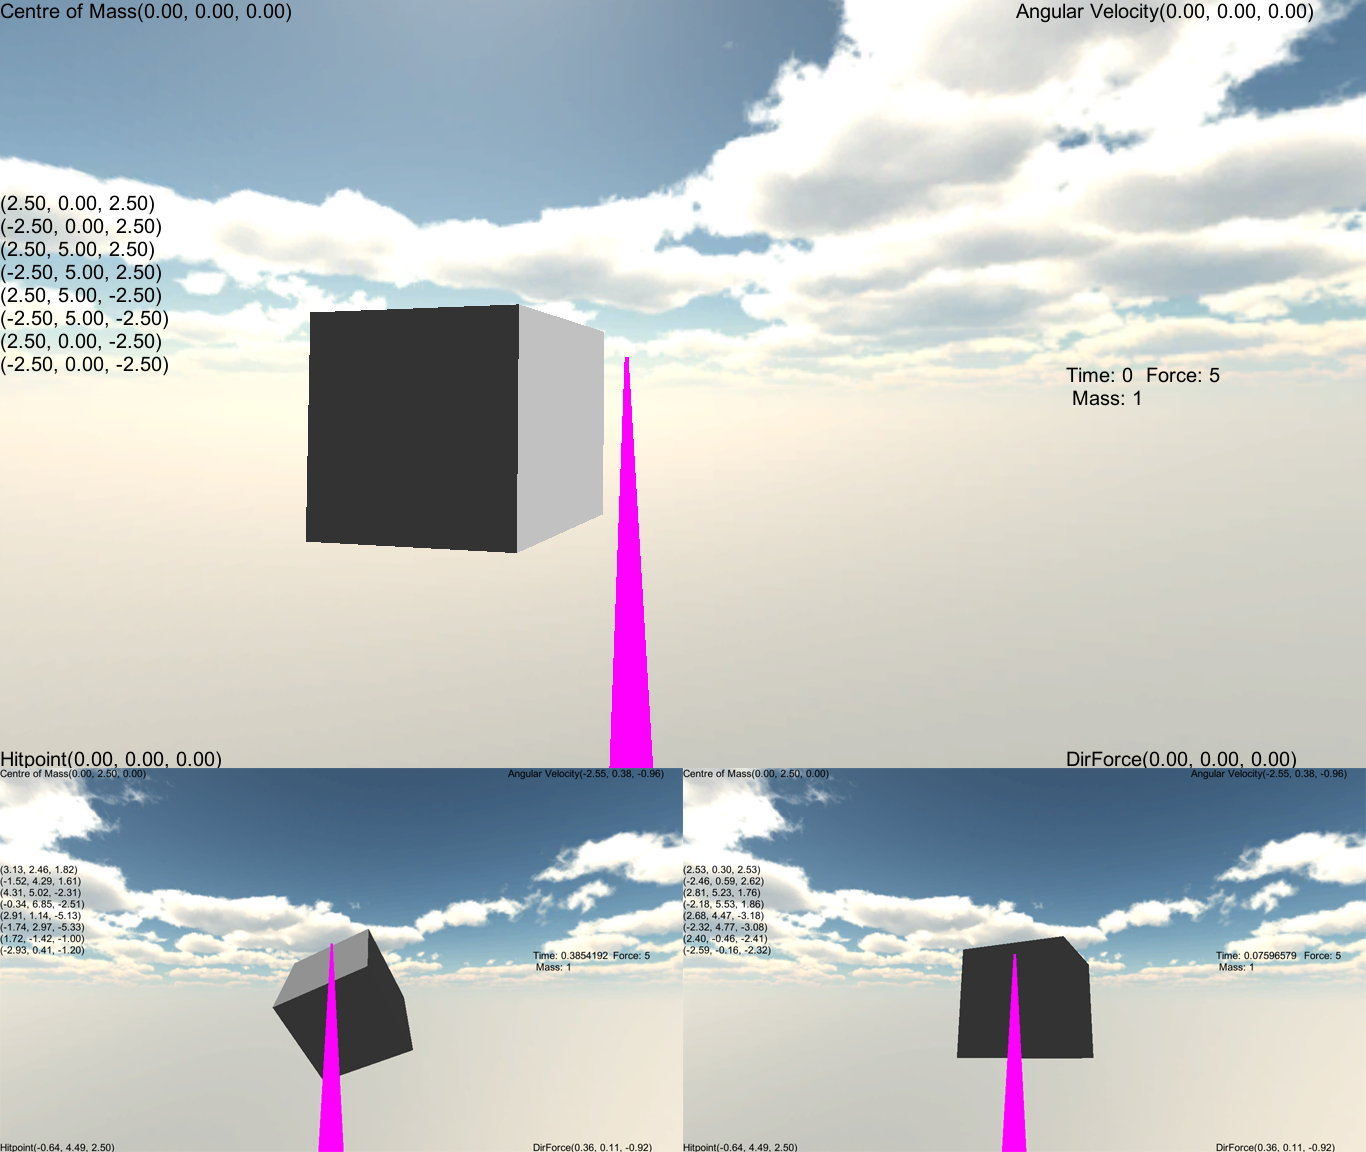
\includegraphics[width=\textwidth]{images/Simulation.PNG}
	\caption{Simulation Screenshots}
	\label{fig:Simulation}
\end{figure}

As seen in Figure \ref{fig:Simulation} the application outputs the location of the centre of mass at the top right of the screen as well as the position of the 8 vertices just below this.
At the bottom left hand side of the screen the user can see the vector for the position at which the force is applied to on the object.
While on the other side of the screen at the top right the angular velocity is outputted once it is calculated by Unity3D.
At the middle of the right hand side of the screen are three variables needed for calculating the motion of rigid bodies; time, force, and mass.
Time here is displayed in seconds, mass in kilograms, and force is displayed in newtons.
The bottom right hand of the screen displays the direction the force is applied in.